\documentclass[12pt]{article}
\usepackage{graphicx}
\usepackage[margin=30mm, paper = a4paper]{geometry}
\usepackage{minted, caption}
\usepackage{subcaption}
\usepackage{multicol}

\title{}
\author{}
\date{}
\setlength{\columnseprule}{1pt}
\setlength{\columnsep}{2cm}
\begin{document}
\vspace*{\fill}
\begin{center}

    \emph{Heaven's Light is Our Guide} \\
    \textbf{Rajshahi University of Engineering and Technology} \\

    \begin{figure}[h]
        \centering
        
\includegraphics[scale=.34]{images/RUET_logo.png}
        \label{fig:ruet_logo}
    \end{figure}
    \vspace{5mm}

    \textbf{Course Code}\\
    ECE 2216\\
    \vspace{3mm}
    \textbf{Course Title}\\
    Database Systems Sessional

    \vspace{5mm}
    \textbf{Experiment Date:} October 15, 2023,\\
    \textbf{Submission Date:} November 5, 2023\\

    \vspace{5mm}
    \textbf{Lab Report 3:} Creating a database and doing operations on it using SQL\\

    \vspace{15mm}

    \begin{tabular}{c|c}
        \textbf{Submitted to} & \textbf{Submitted by} \\
        Md. Robiul Islam      & Md. Tajim An Noor     \\
        Assistant Professor   & Roll: 2010025         \\
        Dept of ECE, Ruet     &                       \\
    \end{tabular}

\end{center}
\vspace*{\fill}

\pagebreak

\tableofcontents

\maketitle

\section{Tools Used}
\begin{itemize}
    \item MySQL
    \item VS Code - as an IDE to use SQL
    \item MacTeX -\LaTeX  compiler
    \item VS Code with LaTeX workshop extension as a text editor
\end{itemize}


\section{Process}

\subsection*{SQL Codes:}
\subsubsection{Find the person who is the top of the organisation (i.e. reports to no one).}
\subsubsection*{Code:}
\begin{minted}[breaklines, linenos]{mysql}
SELECT
    *
FROM
    employees
WHERE
    reportsTo IS NULL;
\end{minted}
\vspace{10mm}

\subsubsection{Find the difference in days between the most recent and oldest order date in Orders file.}
\subsubsection*{Code: }
\begin{minted}[breaklines, linenos]{mysql}
SELECT
    datediff(max(orderDate), min(orderDate))
FROM
    orders;
\end{minted}

\vspace{10mm}

\subsubsection{Find the value of  payments received in July 2004.}
\subsubsection*{Code: }
\begin{minted}[breaklines, breakanywhere, linenos]{mysql}
SELECT
    sum(amount)
FROM
    payments
WHERE
    YEAR(paymentDate) = 2004
    and MONTH(paymentDate) = 7;
\end{minted}
\vspace{10mm}

\subsubsection{Compute the profit generated by each sales representative based on the orders from the customers they serve. Sort by profit generated descending.}
\subsubsection*{Code: }
\begin{minted}[breaklines, breakanywhere, linenos]{mysql}
SELECT
    concat(e.firstName, ' ', e.lastName),
    e.jobTitle,
    SUM(od.quantityOrdered *(od.priceEach - p.buyPrice)) AS totalProfit
FROM
    employees e
    JOIN customers c ON e.employeeNumber = c.salesRepEmployeeNumber
    JOIN orders o USING(customerNumber)
    JOIN orderdetails od USING(orderNumber)
    JOIN products p USING(productCode)
GROUP BY
    e.employeeNumber
ORDER BY
    SUM(od.quantityOrdered *(od.priceEach - p.buyPrice)) DESC;
\end{minted}
\vspace{10mm}

\subsubsection{Find the products sold in 2003 but not 2004.}
\subsubsection*{Code:}
\begin{minted}[linenos,breaklines,breakanywhere]{mysql}
SELECT
    shippedDate,
    productCode,
    productName
FROM
    orders o
    JOIN orderdetails od USING(orderNumber)
    JOIN products p USING(productCode)
GROUP BY
    shippedDate,
    productCode,
    productName
HAVING
    YEAR(o.shippedDate) = 2003
ORDER BY
    shippedDate ASC;
\end{minted}

\vspace{5mm}
\subsubsection{Report the number of orders ‘On Hold’ for each customer.}
\subsubsection*{Code:}
\begin{minted}[linenos,breaklines,breakanywhere]{mysql}
SELECT
    COUNT(orderNumber)
FROM
    orders
WHERE
    status = 'On Hold';
\end{minted}

\vspace{5mm}
\subsubsection{The names of products sold at less than 80\% of the MSRP.}
\subsubsection*{Code:}
\begin{minted}[linenos,breaklines,breakanywhere]{mysql}
SELECT
    productCode,
    priceEach,
    MSRP
FROM
    products
    JOIN orderdetails USING(productCode)
WHERE
    priceEach < 0.8 * MSRP
\end{minted}
\pagebreak
\section{Output}
\captionsetup{justification=centering}
\begin{figure}[htbp!]
    \begin{subfigure}{1\textwidth}
        \centering
        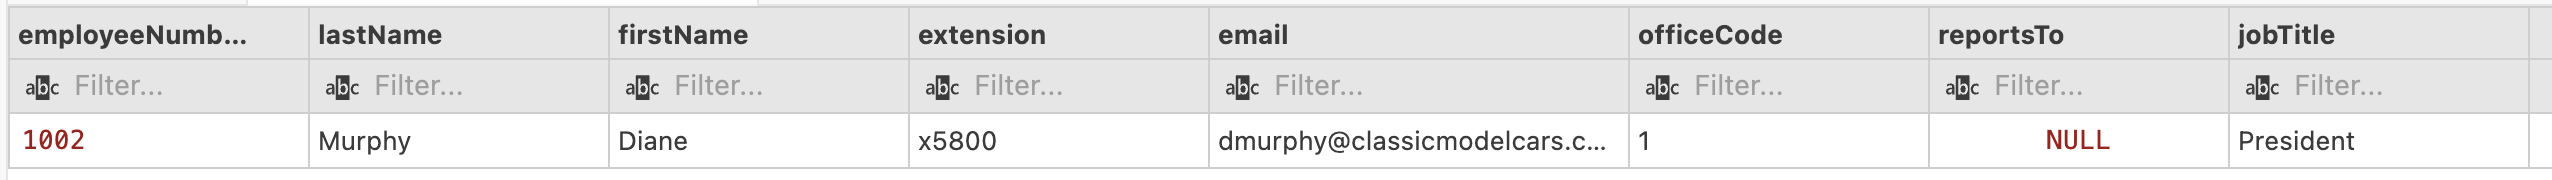
\includegraphics[width=\linewidth]{images/output/q1.png}
        \caption*{The person who is the top of the organization (i.e. reports to no one)}
        \label{fig:q1}
    \end{subfigure}
    \vspace*{20mm}
    \begin{subfigure}{.3\textwidth}
        \centering
        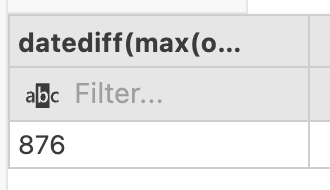
\includegraphics[width=.6\linewidth]{images/output/q2.png}
        \caption*{Difference in days between the most recent and oldest order date in Orders file.}
        \label{fig:q2}
    \end{subfigure}
    \begin{subfigure}{.3\textwidth}
        \centering
        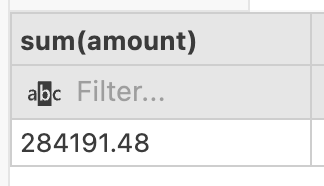
\includegraphics[width=.6\linewidth]{images/output/q3.png}
        \caption*{Total value of  payments received in July 2004.}
        \label{fig:q3}
    \end{subfigure}
    \begin{subfigure}{.3\textwidth}
        \centering
        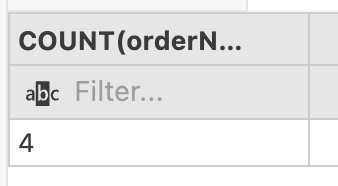
\includegraphics[width=.6\linewidth]{images/output/q6.png}
        \caption*{The number of orders ‘On Hold’ for each customer.}
        \label{fig:q6}
    \end{subfigure}

    \begin{subfigure}{\textwidth}
        \centering
        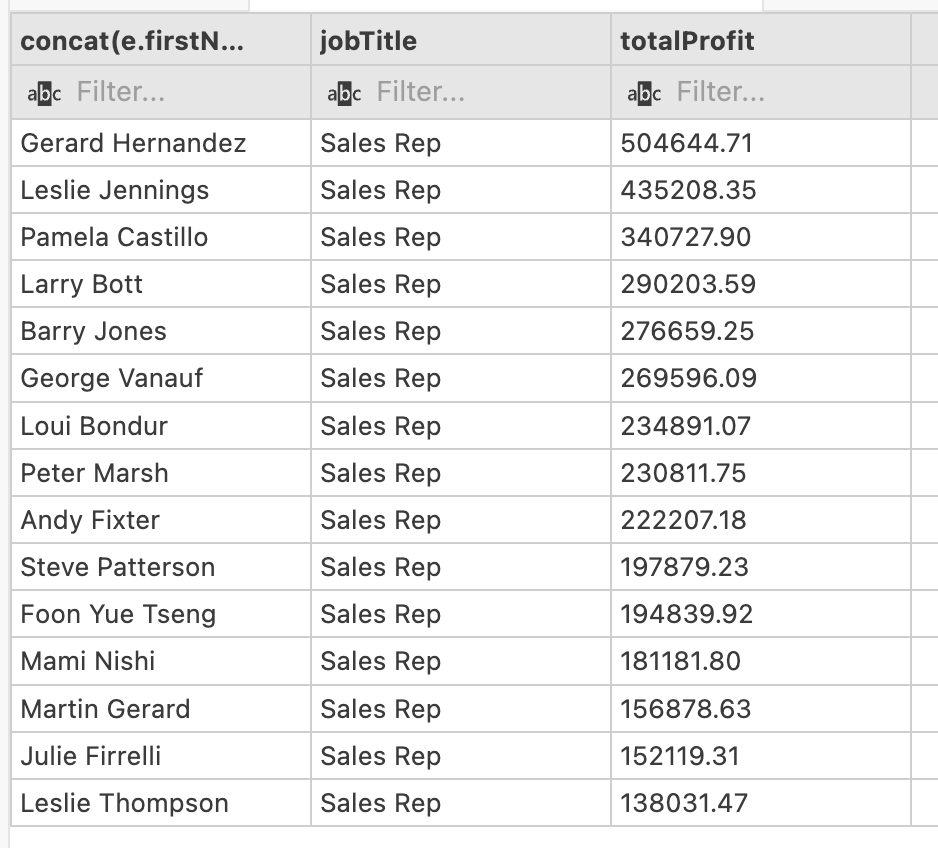
\includegraphics[width=.5\linewidth]{images/output/q4.png}
        \caption*{Profit generated by each sales representative based on the orders from the customers they serve. Sorted by profit generated descending.}
        \label{fig:q4}
    \end{subfigure}
    \begin{subfigure}{.5\textwidth}
        \centering
        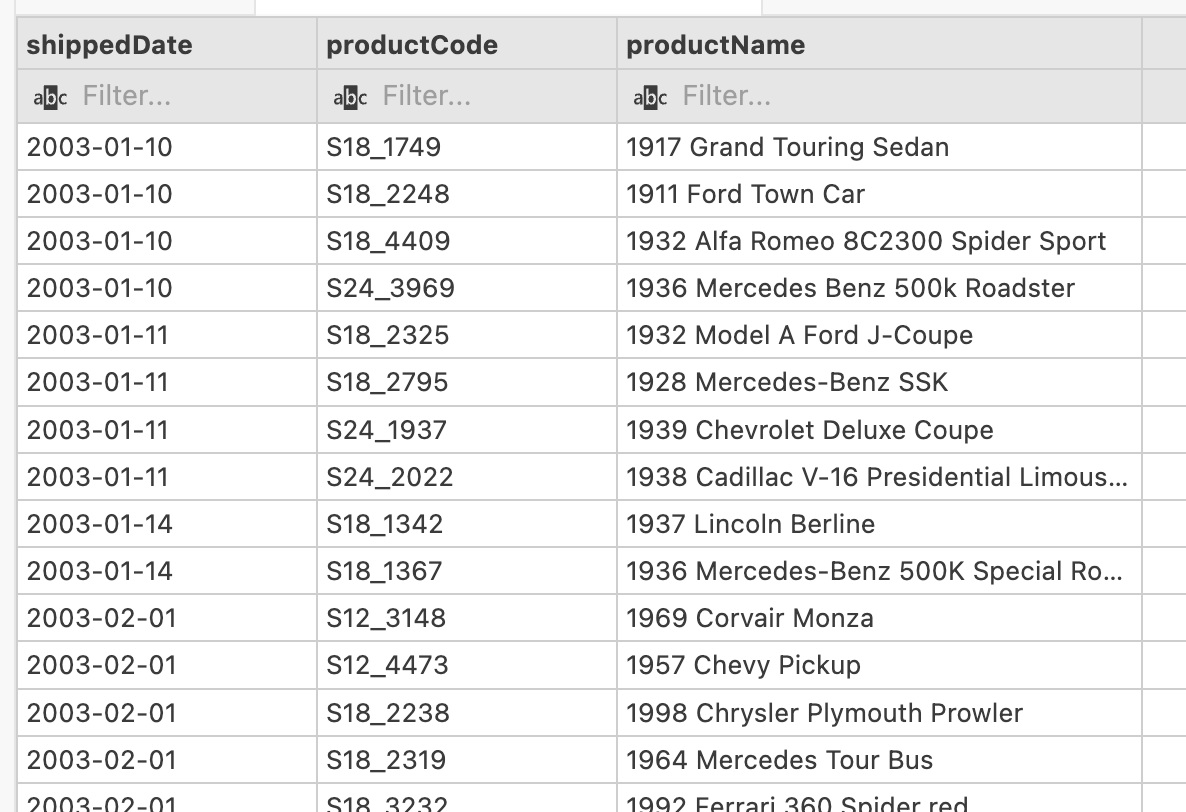
\includegraphics[width=.8\linewidth]{images/output/q5.png}
        \caption*{Products sold in 2003 but not 2004.}
        \label{fig:q5}
    \end{subfigure}
    \begin{subfigure}{.5\textwidth}
        \centering
        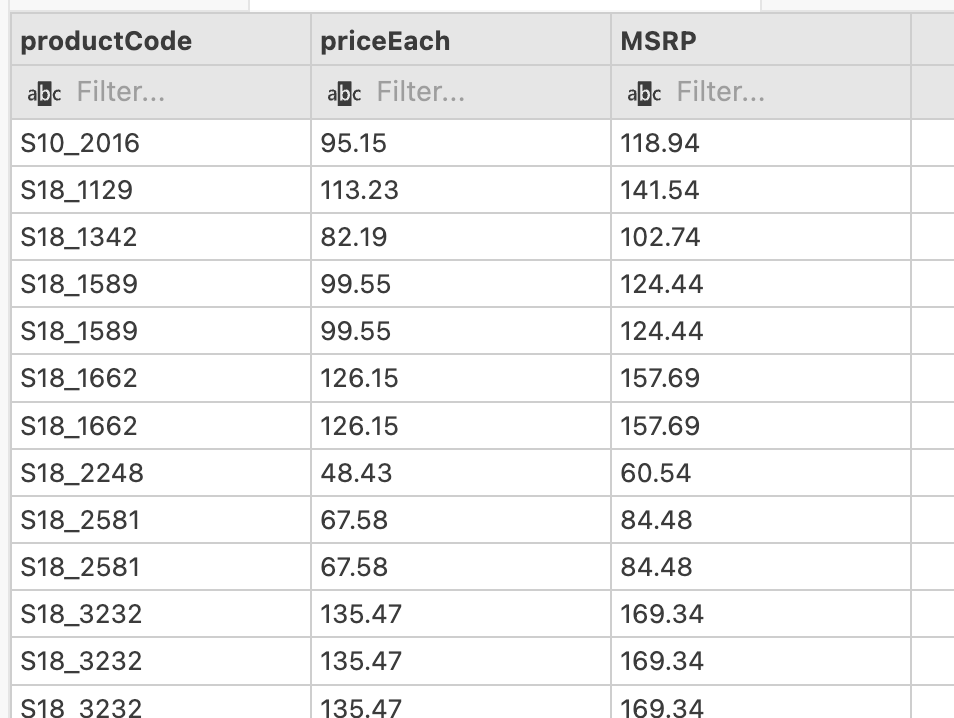
\includegraphics[width=.65\linewidth]{images/output/q7.png}
        \caption*{Names of products sold at less than 80\% of the MSRP.}
        \label{fig:q7}
    \end{subfigure}
\end{figure}

\end{document}